\chapter{Escoamentos viscosos}\label{ch:b2:viscous-flows}

Incline um pote de mel e ele escorre numa fita lenta e espessa; incline
um copo de água e ela some. Passe uma colher por cada um: o mel resiste,
e continua resistindo a qualquer velocidade; a água mal reage até que
você se apresse, e então ela se revolve. A diferença é a \emph{\omterm{def:b2:viscous-flows:viscosity}{viscosidade}} ---
o atrito interno de um fluido --- e a disputa entre \omterm{def:b2:viscous-flows:viscosity}{viscosidade}
e inércia, resumida num único número, o de Reynolds, decide se um
escoamento rasteja em camadas ordenadas ou desaba em turbulência. Este capítulo
acrescenta a força viscosa à \omterm{thm:b2:euler-bernoulli:euler}{equação de Euler}, resolve os dois \omterm{def:b2:viscous-flows:reynolds}{escoamentos
laminares} que todo engenheiro usa e explica por que, a alto \omterm{def:b2:viscous-flows:reynolds}{número de Reynolds},
a \omterm{def:b2:viscous-flows:viscosity}{viscosidade} se esconde numa fina camada junto à parede e ainda assim custa a todo
carro, navio e avião a maior parte de seu combustível.

\begin{omfigure}
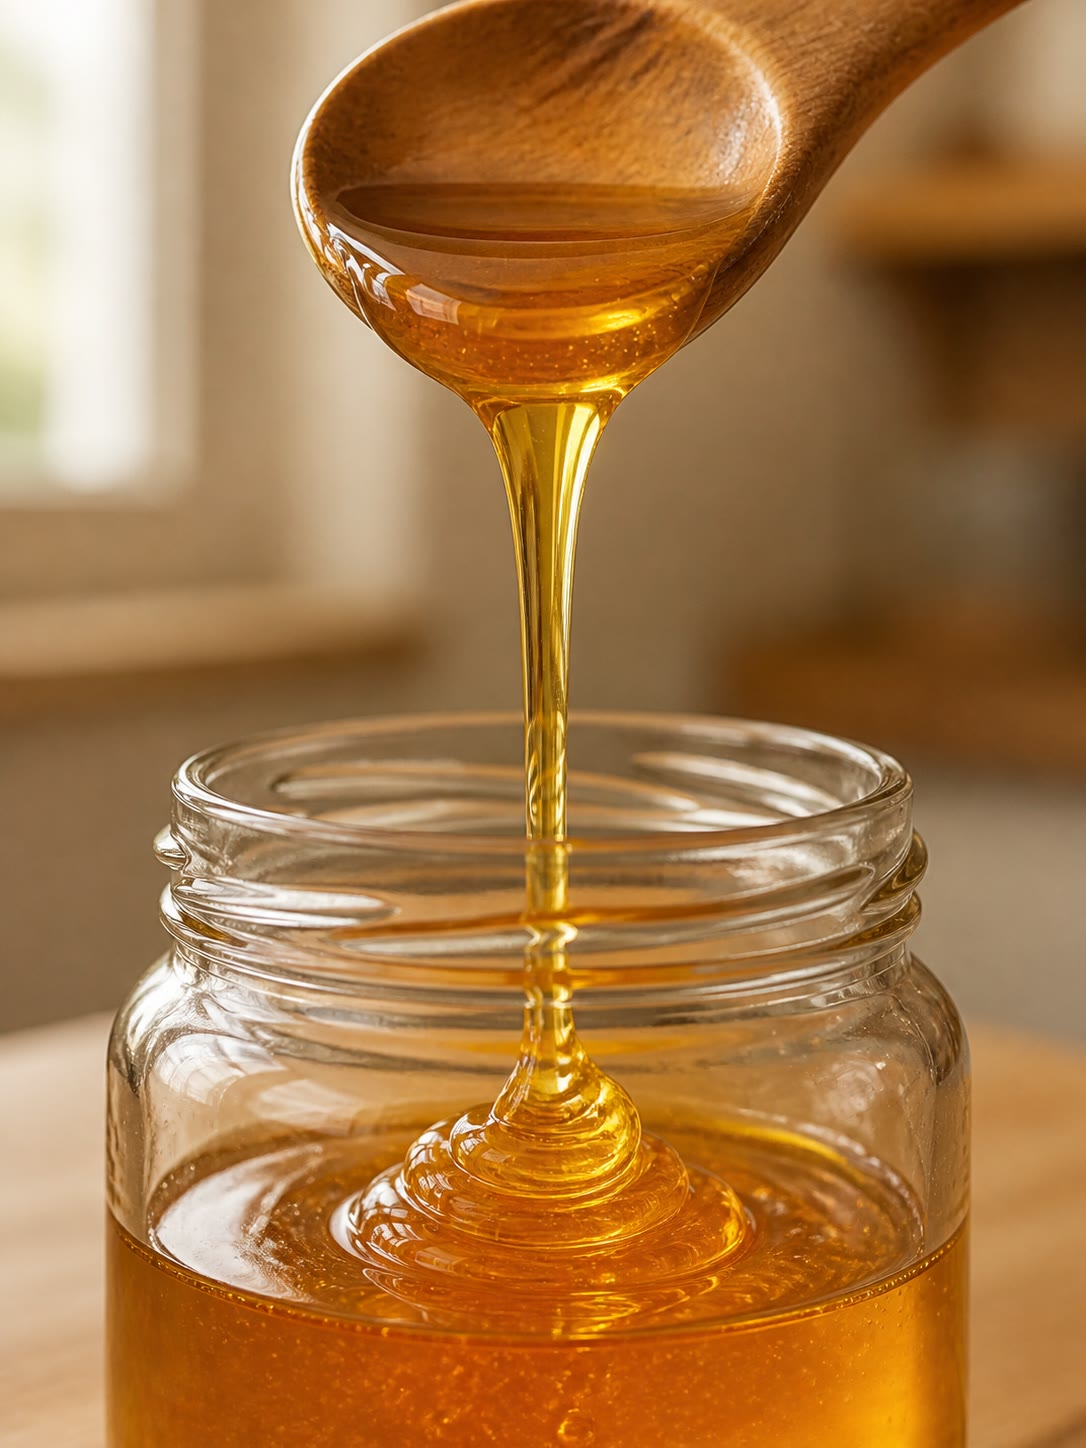
\includegraphics[width=0.34\linewidth]{images/book4/ai/b4-04-honey-spoon-viscous.jpg}

{\small O mel escorre numa fita fina e regular que se enrola ao chegar: uma \omterm{def:b2:viscous-flows:viscosity}{viscosidade} dez mil vezes a da água torna a inércia irrelevante --- é um escoamento rastejante.}
\end{omfigure}


\section{Viscosidade e a equação de Navier--Stokes}

\begin{definition}[Viscosidade newtoniana]\label{def:b2:viscous-flows:viscosity}
\index{viscosidade}\index{viscosidade dinâmica}\index{viscosidade cinemática}\index{tensão de cisalhamento}\index{fluido newtoniano}
Num cisalhamento plano $\vect v = v_x(y)\,\vect e_x$, o fluido acima de uma
superfície $y = $ const. exerce sobre o fluido de baixo (através de um elemento
de superfície $\dd S$) a força tangencial
\[
\dd\vect F = \eta\,\frac{\dd v_x}{\dd y}\,\dd S\;\vect e_x ,
\]
arrastando para a frente a camada mais lenta e sendo, em troca, puxado para trás.
A \emph{tensão de cisalhamento} vale $\tau = \eta\,\dd v_x/\dd y$; o coeficiente
$\eta$ (unidade \unit{Pa.s}) é a \emph{viscosidade dinâmica} do fluido,
e $\nu = \eta/\rho$ (\unit{m^2/s}) sua \emph{viscosidade cinemática}. Um fluido
para o qual $\eta$ não depende da taxa de cisalhamento é \emph{newtoniano}:
água, ar, óleos, álcool; sangue, tinta, ketchup e polímeros fundidos não
são. Ordens de grandeza a \qty{20}{\degreeCelsius}: ar $\eta =
\qty{1.8e-5}{Pa.s}$ ($\nu = \qty{1.5e-5}{m^2/s}$), água $\qty{1.0e-3}{Pa.s}$
($\nu = \qty{1.0e-6}{m^2/s}$), azeite $\qty{0.08}{Pa.s}$, glicerol
$\qty{1.5}{Pa.s}$, mel $\sim\qty{10}{Pa.s}$. Os líquidos ficam mais fluidos quando
aquecidos, e os gases mais viscosos.
\end{definition}

\begin{proposition}[Densidade de força viscosa; condição de aderência]\label{prop:b2:viscous-flows:density}
\index{condição de aderência}\index{densidade de força viscosa}
No cisalhamento plano, a força viscosa resultante sobre uma fatia de fluido
entre $y$ e $y + \dd y$ vale, por unidade de volume, $\eta\,\dd^2v_x/\dd y^2$:
a \omterm{def:b2:viscous-flows:viscosity}{viscosidade} age como uma densidade volumétrica de força $\eta\,\Delta\vect v$ (o
laplaciano tomado componente a componente), resultado que vale para qualquer
\omterm{cor:b2:fluid-kinematics:incompressible}{escoamento incompressível}. Numa parede sólida o fluido \emph{adere}: sua
velocidade é a da parede (a \emph{\omterm{prop:b2:viscous-flows:density}{condição de aderência}}), e é por isso que
a poeira fica na pá de um ventilador e que uma parede sente um arrasto viscoso.
\end{proposition}

\begin{proof}
A fatia é puxada por $\eta\,v_x'(y + \dd y)\dd S$ por cima e por
$-\eta\,v_x'(y)\dd S$ por baixo: resultante $\eta v_x''\,\dd y\,\dd S$. A forma
geral é admitida (segue de escrever a tensão como função linear
simétrica dos gradientes de velocidade). A \omterm{prop:b2:viscous-flows:density}{condição de aderência} é
experimental.
\end{proof}

\begin{theorem}[Equação de Navier--Stokes]\label{thm:b2:viscous-flows:ns}
\index{equação de Navier--Stokes}
Um \omterm{def:b2:viscous-flows:viscosity}{fluido newtoniano} incompressível obedece a
\[
\rho\Bigl(\frac{\partial\vect v}{\partial t} + (\vect v\cdot\operatorname{\vect{grad}})
\vect v\Bigr) = -\operatorname{\vect{grad}}P + \rho\vect g + \eta\,\Delta\vect v ,
\qquad \operatorname{div}\vect v = 0 ,
\]
com a \omterm{prop:b2:viscous-flows:density}{condição de aderência} em toda parede. A \omterm{thm:b2:euler-bernoulli:euler}{equação de Euler} é o caso
$\eta = 0$.
\end{theorem}
\admitted

\begin{omfigure}
\begin{tikzpicture}[font=\small, x=1cm, y=1cm, >=Stealth]
  \begin{scope}
    \draw[thick] (-0.2,0) -- (3.6,0); \fill[pattern=north east lines] (-0.2,-0.18) rectangle (3.6,0);
    \draw[thick, omExo] (-0.2,2.2) -- (3.6,2.2); \fill[pattern=north east lines, pattern color=omExo] (-0.2,2.2) rectangle (3.6,2.38);
    \draw[omExo, very thick, ->] (1.4,2.6) -- (2.6,2.6) node[right, font=\footnotesize] {$U$};
    \foreach \y in {0.4,0.8,...,2.0} \draw[omDef, thick, ->] (0.4,\y) -- ({0.4+1.1*\y/2.2*1.8},\y);
    \draw[omDef, thick] (0.4,0) -- (2.2,2.2);
    \node[font=\footnotesize] at (1.8,-0.5) {Couette: $v_x = Uy/h$, $\tau = \eta U/h$};
    \draw[<->] (3.3,0) -- (3.3,2.2) node[midway, right, font=\footnotesize] {$h$};
  \end{scope}
  \begin{scope}[xshift=7.2cm]
    \draw[thick, fill=omDef!10] (0,0.6) rectangle (3.0,1.6);
    \draw[omThm, very thick, ->] (1.5,1.6) -- (2.6,1.6) node[above, font=\footnotesize] {$\eta v_x'(y+\dd y)\,\dd S$};
    \draw[omThm, very thick, ->] (1.5,0.6) -- (0.4,0.6) node[below, font=\footnotesize] {$\eta v_x'(y)\,\dd S$};
    \node[font=\footnotesize] at (-0.5,1.6) {$y + \dd y$};
    \node[font=\footnotesize] at (-0.4,0.6) {$y$};
    \node[font=\footnotesize] at (1.5,-0.5) {resultante: $\eta\,v_x''\,\dd y\,\dd S$};
  \end{scope}
\end{tikzpicture}

{\small À esquerda: escoamento de Couette plano entre uma placa fixa e uma placa
que se move a $U$ --- perfil linear, e a mesma \omterm{def:b2:viscous-flows:viscosity}{tensão de cisalhamento} em cada
camada. À direita: as forças viscosas sobre uma fatia de fluido; elas se cancelam a menos que
o perfil de velocidades seja curvo.}
\end{omfigure}

\begin{example}[Tensão de cisalhamento sobre uma mesa]\label{ex:b2:viscous-flows:table}
Um filme de \qty{0.1}{mm} de óleo ($\eta = \qty{0.1}{Pa.s}$) entre uma placa e uma
mesa, com a placa deslizando a \qty{1}{m/s}: $\tau = \eta U/h = \qty{1}{kPa}$, uma
força de \qty{100}{N} sobre um décimo de metro quadrado --- é o princípio do
\omterm{def:b2:rigid-body-mechanics:pivot}{mancal} lubrificado, em que o arrasto viscoso substitui um atrito seco
cem vezes maior. Mel numa colher, \qty{10}{Pa.s}, com \qty{1}{mm} de espessura,
escorrendo a \qty{1}{mm/s}: $\tau = \qty{10}{Pa}$, exatamente o peso de um
milímetro de mel por unidade de área --- e é por isso que ele escorre nessa velocidade.
\end{example}

\section{O número de Reynolds}

\begin{definition}[Número de Reynolds]\label{def:b2:viscous-flows:reynolds}
\index{número de Reynolds}\index{escoamento laminar}\index{escoamento turbulento}
Para um escoamento de celeridade característica $U$ e comprimento característico $L$, o \emph{número
de Reynolds}
\[
\mathrm{Re} = \frac{\rho UL}{\eta} = \frac{UL}{\nu}
\]
é a razão entre as ordens de grandeza do termo inercial
$\rho(\vect v\cdot\operatorname{\vect{grad}})\vect v \sim \rho U^2/L$ e do
termo viscoso $\eta\Delta\vect v \sim \eta U/L^2$ na \omterm{thm:b2:viscous-flows:ns}{equação de
Navier--Stokes}. Com $\mathrm{Re} \ll 1$ a inércia é desprezível e o escoamento é
\emph{rastejante} (viscoso, reversível, suave); com $\mathrm{Re} \gg 1$
a \omterm{def:b2:viscous-flows:viscosity}{viscosidade} é desprezível fora das paredes e o escoamento é o de um
\omterm{def:b2:euler-bernoulli:perfect}{fluido perfeito} --- até que, além de um limiar da ordem de $10^3$ (cerca de $2000$
a $3000$ num tubo, baseado no diâmetro), ele se torne \emph{turbulento}:
não permanente, caótico, cheio de turbilhões em todas as escalas. Entre os dois, um
escoamento é \emph{laminar}: permanente e em camadas.
\end{definition}

\begin{example}[Números de Reynolds do cotidiano]\label{ex:b2:viscous-flows:revalues}
Uma bactéria (\qty{1}{\micro m}, \qty{30}{\micro m/s}, em água): $\mathrm{Re} =
3 \times 10^{-5}$ --- ela vive num mundo sem inércia, onde parar
o flagelo a detém em um diâmetro atômico. Sangue num capilar:
$10^{-3}$; um grão de poeira caindo: $10^{-2}$; um peixinho dourado: $10^3$; um nadador:
$10^6$; um carro a \qty{30}{m/s} (\qty{4}{m}): $8 \times 10^6$; um avião de linha: $10^8$;
a Corrente do Golfo: $10^{11}$. Dois escoamentos de mesma geometria e mesmo
\omterm{def:b2:viscous-flows:reynolds}{número de Reynolds} são \emph{semelhantes}: é isso que permite ensaiar um modelo de navio de \qty{1}{m}
num tanque de reboque, ou um avião num túnel de vento.
\end{example}

\section{Escoamentos laminares: Couette, Poiseuille, Stokes}

\begin{proposition}[Escoamento de Poiseuille num tubo]\label{prop:b2:viscous-flows:poiseuille}
\index{escoamento de Poiseuille}\index{resistência hidráulica}
Num tubo cilíndrico horizontal de raio $R$ e comprimento $L$, impulsionado pela
diferença de pressão $\Delta P = P_1 - P_2$ entre suas extremidades, o \omterm{def:b2:viscous-flows:reynolds}{escoamento
laminar} permanente é
\[
v(r) = \frac{\Delta P}{4\eta L}\,(R^2 - r^2) , \qquad
D_V = \frac{\pi R^4}{8\eta L}\,\Delta P :
\]
um perfil parabólico, máximo no eixo, com celeridade média
$\langle v\rangle = v_{\max}/2$. A vazão é proporcional à
queda de pressão (lei de Poiseuille), com a \emph{\omterm{prop:b2:viscous-flows:poiseuille}{resistência hidráulica}}
$R_h = \Delta P/D_V = 8\eta L/\pi R^4$ --- e à \emph{quarta potência} do
raio. A \omterm{def:b2:viscous-flows:viscosity}{tensão de cisalhamento} na parede vale $\tau_w = \Delta P\,R/2L = 4\eta\langle v
\rangle/R$. Válido enquanto $\mathrm{Re} = 2R\langle v\rangle/\nu \lesssim 2000$.
\end{proposition}

\begin{proof}
Permanente, $\vect v = v(r)\vect e_z$ (de modo que o termo convectivo se anula: $\vect v
\cdot\operatorname{\vect{grad}}$ age ao longo de $z$, direção em que nada
varia). Navier--Stokes ao longo de $z$: $0 = -\partial_zP + \eta\Delta v$, e
radialmente $\partial_rP = 0$: $P$ só depende de $z$, e $\Delta v$ só de $r$, de modo que
ambos os lados valem uma constante, $\partial_zP = -\Delta P/L$. Em coordenadas
cilíndricas $\Delta v = \frac1r\frac{\dd}{\dd r}\bigl(r\frac{\dd v}{\dd r}\bigr)$
(enunciado; é o balanço das forças viscosas sobre uma casca cilíndrica,
$2\pi rL\,\eta v'$ em $r$ e em $r + \dd r$). Integrando duas vezes com $v$
finito no eixo e $v(R) = 0$ obtém-se a parábola; $D_V = \int_0^Rv\,2\pi
r\,\dd r$. A tensão na parede é $-\eta v'(R)$; equivalentemente, a força
de pressão $\pi R^2\Delta P$ equilibra o atrito na parede $2\pi RL\tau_w$.
\end{proof}

\begin{omfigure}
\begin{tikzpicture}[font=\small, x=1cm, y=1cm, >=Stealth]
  \begin{scope}
    \draw[thick] (-2.8,1.0) -- (2.8,1.0) (-2.8,-1.0) -- (2.8,-1.0);
    \fill[pattern=north east lines] (-2.8,1.0) rectangle (2.8,1.15); \fill[pattern=north east lines] (-2.8,-1.0) rectangle (2.8,-1.15);
    \draw[omDef, thick, domain=-1:1, samples=40] plot ({-0.9+1.8*(1-\x*\x)},\x);
    \foreach \y in {-0.8,-0.6,...,0.8} \draw[omDef, ->] (-0.9,\y) -- ({-0.9+1.8*(1-\y*\y)-0.05},\y);
    \draw[dashed] (-0.9,-1) -- (-0.9,1);
    \node[omDef, font=\footnotesize] at (1.6,0.3) {$v_{\max}$};
    \node[font=\footnotesize] at (-2.3,0.0) {$P_1$}; \node[font=\footnotesize] at (2.4,0.0) {$P_2$};
    \node[font=\footnotesize] at (0,-1.5) {$v(r) = \dfrac{\Delta P}{4\eta L}(R^2 - r^2)$};
  \end{scope}
  \begin{scope}[xshift=7.6cm]
    \draw[thick] (-2.2,0) -- (2.2,0) (-2.2,0.5) -- (2.2,0.5) (-2.2,-0.5) -- (2.2,-0.5);
    \draw[thick] (-2.2,-0.5) -- (-2.2,0.5) (2.2,-0.5) -- (2.2,0.5);
    \fill[omDef!15] (-2.2,0) rectangle (2.2,0.5);
    \draw[omThm, very thick, ->] (-3.2,0.25) -- (-2.25,0.25) node[pos=0.2, above, font=\footnotesize] {$P_1$};
    \draw[omThm, very thick, ->] (3.2,0.25) -- (2.25,0.25) node[pos=0.2, above, font=\footnotesize] {$P_2$};
    \draw[omProp, very thick, ->] (0.8,0.5) -- (-0.4,0.5) node[above, font=\footnotesize, pos=0.9] {$\tau(r+\dd r)$};
    \draw[omProp, very thick, ->] (-0.4,0.0) -- (0.8,0.0) node[below, font=\footnotesize, pos=0.9] {$\tau(r)$};
    \node[font=\footnotesize] at (0,-1.3) {casca $[r, r + \dd r]$: pressão $=$ arrasto viscoso};
  \end{scope}
\end{tikzpicture}

{\small À esquerda: o \omterm{prop:b2:viscous-flows:poiseuille}{escoamento de Poiseuille} --- o perfil parabólico num tubo,
impulsionado pela queda de pressão $P_1 - P_2$. À direita: o balanço de forças numa
casca cilíndrica de fluido: a diferença de pressão em suas bases é
equilibrada pelas tensões viscosas em suas superfícies interna e externa.}
\end{omfigure}

\begin{example}[A quarta potência]\label{ex:b2:viscous-flows:fourth}
Uma agulha de seringa de diâmetro interno \qty{0.4}{mm} e comprimento \qty{3}{cm},
com água e pressão do polegar de \qty{20}{kPa}: $D_V = \pi(2 \times 10^{-4})^4 \times 2 \times
10^4/(8 \times 10^{-3} \times 0.03) = \qty{0.42}{mL/s}$; uma agulha duas vezes mais larga
dá dezesseis vezes mais. Uma artéria estreitada por uma placa a $70\%$ de seu
raio oferece $(1/0.7)^4 = 4.2$ vezes a resistência: o corpo compensa
elevando a pressão a montante, o que é parte da razão de aterosclerose
e hipertensão andarem juntas.
\end{example}

\begin{proposition}[Arrasto de Stokes]\label{prop:b2:viscous-flows:stokes}
\index{lei de Stokes}\index{velocidade terminal}\index{sedimentação}
Uma esfera de raio $R$ que se move com celeridade $v$ num fluido a
$\mathrm{Re} = 2\rho vR/\eta \ll 1$ sofre o arrasto
\[
F = 6\pi\eta Rv ,
\]
oposto à sua velocidade. Uma esfera de massa específica $\rho_s$ que cai num fluido
de massa específica $\rho$ atinge a \emph{\omterm{prop:b2:viscous-flows:stokes}{velocidade terminal}} $v_\infty =
\dfrac{2R^2(\rho_s - \rho)g}{9\eta}$ --- a lei da sedimentação, das
centrífugas e das gotas de óleo de Millikan.
\end{proposition}

\begin{proof}
O arrasto é admitido (é a solução exata das equações do escoamento
rastejante em torno de uma esfera, dois terços dele atrito viscoso e um terço
pressão). \omterm{prop:b2:viscous-flows:stokes}{Velocidade terminal}: o peso menos o empuxo, $\tfrac43\pi R^3(\rho_s -
\rho)g$, iguala o arrasto; verifique sempre $\mathrm{Re} \ll 1$ depois.
\end{proof}

\begin{example}[Neblina, chuva e poeira]\label{ex:b2:viscous-flows:fog}
Uma gotícula de neblina de \qty{10}{\micro m} de diâmetro cai no ar a $2 \times (5 \times
10^{-6})^2 \times 10^4/(9 \times 1.8 \times 10^{-5}) = \qty{3}{mm/s}$ ($\mathrm{Re} = 2 \times
10^{-3}$): a menor corrente ascendente a mantém no ar, e é por isso que as nuvens
flutuam. Uma gota de chuva de \qty{1}{mm} daria \qty{30}{m/s} e $\mathrm{Re} \approx 2000$:
Stokes já não se aplica, e o arrasto quadrático da próxima seção
dá os \qty{4}{m/s} observados. Um grão de poeira de \qty{10}{\micro m} ($\rho_s =
\qty{2500}{kg/m^3}$) sedimenta a \qty{8}{mm/s}, um metro em dois minutos ---
poeira mais fina fica em suspensão por horas.
\end{example}

\section{Alto número de Reynolds: camadas limite e arrasto}

\begin{proposition}[A camada limite]\label{prop:b2:viscous-flows:bl}
\index{camada limite}
A alto \omterm{def:b2:viscous-flows:reynolds}{número de Reynolds} o escoamento em torno de um corpo é o de um \omterm{def:b2:euler-bernoulli:perfect}{fluido
perfeito} em toda parte, exceto numa fina \emph{\omterm{prop:b2:viscous-flows:bl}{camada limite}} junto à parede,
na qual a velocidade cai de seu valor externo $U$ a zero (aderência).
Ao longo de uma placa plana sua espessura cresce como
\[
\delta(x) \sim \sqrt{\frac{\nu x}{U}} = \frac{x}{\sqrt{\mathrm{Re}_x}} ,
\qquad \mathrm{Re}_x = \frac{Ux}{\nu} ,
\]
com $x$ a distância ao bordo de ataque; a própria camada torna-se
turbulenta além de $\mathrm{Re}_x \sim 5 \times 10^5$. O atrito viscoso na
parede e o \emph{descolamento} da camada atrás de um corpo rombudo (que
deixa uma esteira turbulenta de baixa pressão) são as duas fontes de arrasto.
\end{proposition}

\begin{proof}
Ordem de grandeza: uma \omterm{def:b2:fluid-kinematics:particle}{partícula de fluido} gasta o tempo $x/U$ percorrendo
a placa, durante o qual a influência da parede se difunde no
fluido --- o termo viscoso $\nu\,\partial^2v/\partial y^2$ é uma difusão de
quantidade de movimento com difusividade $\nu$, que alcança a distância $\sqrt{\nu t}$ no
tempo $t$ (\cref{ch:b2:particle-diffusion}). Logo $\delta \sim \sqrt{\nu x
/U}$. A teoria completa (de Prandtl) é admitida.
\end{proof}

\begin{proposition}[Arrasto a alto número de Reynolds]\label{prop:b2:viscous-flows:drag}
\index{coeficiente de arrasto}\index{crise do arrasto}
O arrasto sobre um corpo de área frontal $S$ que se move a $v$ num fluido
escreve-se
\[
F = \tfrac12\rho v^2\,S\,C_x ,
\]
onde o \emph{\omterm{prop:b2:viscous-flows:drag}{coeficiente de arrasto}} $C_x$ depende da forma e de
$\mathrm{Re}$. Para uma esfera, $C_x = 24/\mathrm{Re}$ com $\mathrm{Re} \ll 1$ (Stokes,
com $\mathrm{Re}$ baseado no diâmetro), depois cerca de $0.4$--$0.5$, quase
constante, de $\mathrm{Re} \approx 10^3$ a $2 \times 10^5$, onde cai
bruscamente para cerca de $0.1$ (a \emph{\omterm{prop:b2:viscous-flows:drag}{crise do arrasto}}: a \omterm{prop:b2:viscous-flows:bl}{camada limite} torna-se
turbulenta, adere por mais tempo à superfície e a esteira encolhe --- as
covinhas de uma bola de golfe a antecipam). Corpos fuselados têm
$C_x \approx 0.05$; um carro, $0.3$; um ciclista, $0.9$; uma placa plana de frente para o escoamento,
$1.2$. A potência necessária para se mover a $v$ vale $Fv \propto v^3$.
\end{proposition}
\admitted

\begin{omfigure}
\begin{tikzpicture}
\begin{axis}[omaxis, axis x line=bottom, axis y line=left, width=8.0cm, height=5.0cm,
    xmode=log, ymode=log, xmin=0.1, xmax=1e7, ymin=0.05, ymax=300,
    xlabel={$\mathrm{Re} = \rho v\,2R/\eta$}, ylabel={$C_x$},
    xlabel style={at={(axis description cs:0.5,-0.12)}, anchor=north},
    ylabel style={at={(axis description cs:-0.12,0.5)}, rotate=90, anchor=south},
    xtick={0.1,10,1000,1e5,1e7}, ytick={0.1,1,10,100}, samples=100]
  \addplot[omThm, thick, domain=0.1:2] {24/x};
  \addplot[omThm, thick, domain=2:1000] {24/x*(1+0.15*x^0.687)};
  \addplot[omThm, thick, domain=1000:2e5] {0.44};
  \addplot[omThm, thick] coordinates {(2e5,0.44) (3.5e5,0.1)};
  \addplot[omThm, thick, domain=3.5e5:1e7] {0.1+0.1*ln(x/3.5e5)/ln(30)};
  \addplot[omDef, dashed, thick, domain=0.1:100] {24/x};
  \node[font=\scriptsize, omDef, anchor=west] at (axis cs:6,40) {$24/\mathrm{Re}$ (Stokes)};
  \node[font=\scriptsize] at (axis cs:1.5e4,0.9) {patamar $\approx 0.45$};
  \node[font=\scriptsize] at (axis cs:1e6,0.06) {crise do arrasto};
\end{axis}
\end{tikzpicture}
\hfill
\begin{tikzpicture}[font=\small, x=1cm, y=1cm, >=Stealth]
  \draw[thick] (0,0) -- (5.0,0); \fill[pattern=north east lines] (0,-0.15) rectangle (5.0,0);
  \draw[omDef, thick, domain=0.05:5.0, samples=40] plot (\x,{0.55*sqrt(\x)});
  \foreach \x in {0.8,2.0,3.6} {
    \foreach \y in {0.1,0.2,...,1.4} {
      \pgfmathsetmacro{\d}{0.55*sqrt(\x)}
      \pgfmathsetmacro{\u}{min(1,\y/\d)}
      \draw[omThm, ->] (\x,\y) -- ({\x+0.9*\u*(2-(\u)*(1))*0.5+0.0},\y);
    }
  }
  \draw[omThm, very thick, ->] (-0.9,1.6) -- (-0.1,1.6) node[above, font=\footnotesize, pos=0.3] {$U$};
  \node[omDef, font=\footnotesize] at (4.2,1.55) {$\delta(x) \sim \sqrt{\nu x/U}$};
  \node[font=\footnotesize] at (2.5,-0.5) {camada limite numa placa plana};
\end{tikzpicture}

{\small À esquerda: o \omterm{prop:b2:viscous-flows:drag}{coeficiente de arrasto} de uma esfera em função do \omterm{def:b2:viscous-flows:reynolds}{número de
Reynolds} (escalas logarítmicas): a \omterm{prop:b2:viscous-flows:stokes}{lei de Stokes} a baixo $\mathrm{Re}$, um patamar perto de
$0.45$ e a \omterm{prop:b2:viscous-flows:drag}{crise do arrasto} perto de $\mathrm{Re} = 2 \times 10^5$. À direita: a
\omterm{prop:b2:viscous-flows:bl}{camada limite} engrossando ao longo de uma placa plana; fora dela o escoamento é
o de um \omterm{def:b2:euler-bernoulli:perfect}{fluido perfeito}.}
\end{omfigure}

\begin{example}[Um ciclista, um carro]\label{ex:b2:viscous-flows:cyclist}
Um ciclista ($SC_x = \qty{0.35}{m^2}$) a \qty{10}{m/s}: $F = 0.5 \times 1.2 \times 100
\times 0.35 = \qty{21}{N}$, $P = \qty{210}{W}$ --- um esforço sustentável; a \qty{15}{m/s}
(\qty{54}{km/h}) seriam \qty{710}{W}, e é por isso que os velocistas pegam vácuo.
Um carro ($SC_x = \qty{0.7}{m^2}$) a \qty{130}{km/h}: \qty{550}{N}, \qty{20}{kW} só contra
o ar --- o consumo de combustível na velocidade de estrada é sobretudo arrasto.
\end{example}

\begin{remark}[Tensão superficial]\label{rem:b2:viscous-flows:capillarity}
\index{tensão superficial}\index{pressão de Laplace}\index{comprimento capilar}
Uma segunda força mora nas fronteiras de um líquido: sua superfície livre
comporta-se como uma membrana esticada de tensão $\gamma$ (\unit{N/m}; água,
\qty{0.072}{N/m}), porque às moléculas da superfície falta metade dos vizinhos.
A pressão dentro de uma gota de raio $R$ excede a pressão externa
da \emph{\omterm{rem:b2:viscous-flows:capillarity}{pressão de Laplace}} $2\gamma/R$ (\qty{1.4}{kPa} numa gota de \qty{0.1}{mm},
\qty{14}{bar} numa de \qty{10}{nm}); a \omterm{rem:b2:viscous-flows:capillarity}{tensão superficial} vence a gravidade abaixo
do \emph{\omterm{rem:b2:viscous-flows:capillarity}{comprimento capilar}} $\sqrt{\gamma/\rho g} = \qty{2.7}{mm}$ para a água ---
o tamanho das gotas de orvalho, do menisco num copo, da ascensão num
tubo capilar ($h = 2\gamma/\rho gr$, Jurin). É por isso que insetos pequenos andam
sobre a água, que os pelos de um pincel se juntam quando molhados e que um
jato líquido se rompe em gotas.
\end{remark}

\begin{method}[Qual regime?]\label{met:b2:viscous-flows:regime}
Antes de qualquer cálculo de escoamento viscoso, calcule $\mathrm{Re}$. Com $\mathrm{Re} \ll 1$:
Stokes e escoamento rastejante, arrasto $\propto v$, quedas de pressão $\propto$ vazão.
Com $\mathrm{Re}$ até $\sim\!2000$ num tubo: laminar, Poiseuille. Acima disso:
turbulento --- Poiseuille subestima muito a perda; use a
lei empírica $\Delta P = \lambda(L/D)\,\tfrac12\rho\langle v\rangle^2$ com $\lambda
\approx 0.3/\mathrm{Re}^{1/4}$ para tubos lisos, e $F = \tfrac12\rho v^2SC_x$ para
corpos. Em todos os casos, verifique depois que o $\mathrm{Re}$ calculado
a partir da resposta concorda com o regime suposto.
\end{method}

\section{Exercícios}

\begin{exercise}[$\star$]\label{exo:b2:viscous-flows:1}
Uma placa de \qty{0.50}{m^2} desliza a \qty{2.0}{m/s} sobre um filme de \qty{0.20}{mm} de óleo
($\eta = \qty{0.25}{Pa.s}$). \omterm{def:b2:viscous-flows:viscosity}{Tensão de cisalhamento}, força sobre a placa, potência
dissipada; compare com o atrito seco ($f = 0.3$) se a placa pesa
\qty{10}{kg}.
\end{exercise}

\begin{exercise}[$\star$]\label{exo:b2:viscous-flows:2}
\omterm{def:b2:viscous-flows:reynolds}{Números de Reynolds} de: (a) uma bactéria de \qty{2}{\micro m} a \qty{30}{\micro m/s} em
água; (b) um nadador (\qty{1.8}{m}, \qty{1.5}{m/s}); (c) um carro (\qty{4}{m},
\qty{30}{m/s}) no ar; (d) o sangue na aorta (\qty{2.5}{cm}, \qty{0.33}{m/s},
$\nu = \qty{3.3e-6}{m^2/s}$); (e) óleo ($\eta = \qty{0.1}{Pa.s}$, $\rho =
\qty{900}{kg/m^3}$) a \qty{0.5}{m/s} num tubo de \qty{1}{cm}. Regime de cada um.
\end{exercise}

\begin{exercise}[$\star$]\label{exo:b2:viscous-flows:3}
A água é empurrada por \qty{20}{kPa} através de uma agulha de \qty{0.40}{mm} (diâmetro interno)
e \qty{3.0}{cm}. Vazão; tempo para injetar \qty{5}{mL}; celeridade máxima
e \omterm{def:b2:viscous-flows:reynolds}{número de Reynolds}; \omterm{def:b2:viscous-flows:viscosity}{tensão de cisalhamento} na parede. E com uma agulha de \qty{0.80}{mm}?
\end{exercise}

\begin{exercise}[$\star$]\label{exo:b2:viscous-flows:4}
\omterm{prop:b2:viscous-flows:stokes}{Velocidades terminais} no ar ($\eta = \qty{1.8e-5}{Pa.s}$) de (a) um grão de pólen de \qty{20}{\micro m}
($\rho_s = \qty{1100}{kg/m^3}$), (b) uma partícula de fumaça de \qty{2}{\micro m}
($\rho_s = \qty{2000}{kg/m^3}$), (c) uma gota de garoa de \qty{0.2}{mm}.
Verifique $\mathrm{Re}$ em cada caso; tempo para cair \qty{1}{m}.
\end{exercise}

\begin{exercise}[$\star\star$]\label{exo:b2:viscous-flows:5}
Uma adutora de diâmetro \qty{30}{cm} conduz \qty{0.10}{m^3/s} ao longo de
\qty{1.0}{km}. (a) Celeridade média e \omterm{def:b2:viscous-flows:reynolds}{número de Reynolds}. (b) Queda de pressão se
a lei de Poiseuille valesse. (c) Queda real com $\lambda = 0.3/\mathrm{Re}^{1/4}$;
razão em relação a (b); potência de bombeamento. (d) A mesma vazão em duas adutoras
paralelas de \qty{21}{cm} (mesma seção total): queda e potência.
\end{exercise}

\begin{exercise}[$\star\star$]\label{exo:b2:viscous-flows:6}
Células de diâmetro \qty{10}{\micro m} e massa específica \qty{1050}{kg/m^3} em água.
(a) Celeridade de sedimentação sob gravidade; tempo para decantar \qty{5}{cm}. (b) Numa
centrífuga a $1000\,g$. (c) Frequência de rotação mínima para $1000\,g$ a
\qty{10}{cm} de raio. (d) Por que as partículas maiores podem ser separadas primeiro?
\end{exercise}

\begin{exercise}[$\star\star$]\label{exo:b2:viscous-flows:7}
Um ciclista ($SC_x = \qty{0.35}{m^2}$, resistência ao rolamento de \qty{4}{N}) anda a
\qty{12}{m/s}. (a) Arrasto e potência total. (b) A \qty{15}{m/s}. (c) Contra um
vento de proa de \qty{5}{m/s}, a \qty{12}{m/s} em relação ao solo. (d) Pegar vácuo reduz
$C_x$ em $30\%$: potência economizada. (e) Descendo uma rampa de $5\%$ sem pedalar
(massa de \qty{80}{kg}): celeridade terminal.
\end{exercise}

\begin{exercise}[$\star\star$]\label{exo:b2:viscous-flows:8}
Arrasto quadrático. (a) Celeridade terminal de uma bola de golfe (\qty{46}{g}, \qty{43}{mm},
$C_x = 0.25$) e de um paraquedista (\qty{80}{kg}, $SC_x = \qty{0.7}{m^2}$, e depois
$\qty{25}{m^2}$ com o paraquedas aberto). (b) Equação do movimento de uma queda
a partir do repouso com arrasto quadrático; mostre que $v = v_\infty\tanh(gt/v_\infty)$. (c)
Tempo e distância para o paraquedista atingir $90\%$ de $v_\infty$.
\end{exercise}

\begin{exercise}[$\star\star$]\label{exo:b2:viscous-flows:9}
\emph{Viscosímetro de Couette.} Um cilindro de raio \qty{5.0}{cm} e altura
\qty{10}{cm} gira a \qty{10}{rad/s} dentro de um cilindro fixo, com a folga de
\qty{1.0}{mm} preenchida pelo líquido a ensaiar; o torque necessário é
\qty{2.0e-2}{N.m}. (a) Tratando a folga como escoamento de Couette plano, taxa de cisalhamento
e \omterm{def:b2:viscous-flows:viscosity}{tensão de cisalhamento}. (b) \omterm{def:b2:viscous-flows:viscosity}{Viscosidade}. (c) \omterm{def:b2:viscous-flows:reynolds}{Número de Reynolds} do escoamento na folga;
o escoamento é laminar? (d) Por que a folga é feita estreita?
\end{exercise}

\begin{exercise}[$\star\star\star$]\label{exo:b2:viscous-flows:10}
\emph{Uma rede vascular.} O sangue ($\eta = \qty{3.5}{mPa.s}$) escoa a
\qty{5.0}{L/min}. (a) \omterm{prop:b2:viscous-flows:poiseuille}{Resistência hidráulica} da aorta (raio \qty{1.25}{cm},
comprimento \qty{40}{cm}) e queda de pressão ao longo dela. (b) Os $10^{10}$
capilares (raio \qty{4}{\micro m}, comprimento \qty{1}{mm}) estão em paralelo:
resistência de um, de todos, e queda de pressão no leito
capilar. (c) As arteríolas ($10^8$, raio \qty{10}{\micro m}, comprimento
\qty{2}{mm}): mesmas perguntas; onde está a resistência da circulação?
(d) A queda total vale \qty{13}{kPa}: potência do ventrículo esquerdo
e que fração dos \qty{100}{W} do corpo ela representa. (e) Um medicamento dilata as
arteríolas em $10\%$: efeito sobre a resistência total.
\end{exercise}

\begin{exercise}[$\star\star\star$]\label{exo:b2:viscous-flows:11}
\emph{\omterm{prop:b2:viscous-flows:bl}{Camada limite} e arrasto de atrito.} Uma placa plana de comprimento $L$ e
largura $b$ move-se de perfil a $U$. No regime laminar a \omterm{def:b2:viscous-flows:viscosity}{tensão de cisalhamento}
na parede vale $\tau_w = 0.332\,\rho U^2/\sqrt{\mathrm{Re}_x}$ (Blasius). (a) Mostre que
a \omterm{def:b2:rigid-body-mechanics:contact}{força de atrito} numa das faces vale $F = 0.664\,\rho U^2bL/\sqrt{\mathrm{Re}_L}$.
(b) Espessura da \omterm{prop:b2:viscous-flows:bl}{camada limite} no bordo de fuga de uma placa de \qty{1}{m}
em água a \qty{0.3}{m/s}, e força sobre uma placa de \qty{1}{m^2} (nas duas
faces). (c) A \qty{10}{m/s}: $\mathrm{Re}_L$, e por que a fórmula deixa de
valer. (d) Casco de um navio (\qty{100}{m}, \qty{10}{m/s}): estimativa da espessura
da \omterm{prop:b2:viscous-flows:bl}{camada limite} na popa, supondo a lei turbulenta $\delta \approx
0.37x/\mathrm{Re}_x^{1/5}$.
\end{exercise}

\begin{exercise}[$\star\star\star$]\label{exo:b2:viscous-flows:12}
\emph{Um filme que escorre.} Um filme líquido de espessura $h$ escorre por uma
parede vertical sob a gravidade, em regime permanente, sem que o ar exerça tensão em
sua superfície livre. (a) Escreva Navier--Stokes para $\vect v = v(y)\vect e_z$ ($y$
a distância à parede, $z$ para baixo) e as condições de contorno.
(b) Mostre que $v(y) = \dfrac{\rho g}{2\eta}(2hy - y^2)$ e calcule a vazão
por unidade de largura $q = \rho gh^3/3\eta$. (c) Uma demão fresca de tinta ($\eta =
\qty{0.5}{Pa.s}$, $\rho = \qty{1200}{kg/m^3}$) de \qty{0.2}{mm} de espessura: celeridade
da superfície e vazão; quanto a superfície anda em \qty{10}{min}? Por que
a tinta escorre quando aplicada grossa demais? (d) Mel ($\eta = \qty{10}{Pa.s}$)
com \qty{2}{mm} de espessura numa colher vertical: celeridade da superfície.
\end{exercise}

\begin{omfigure}
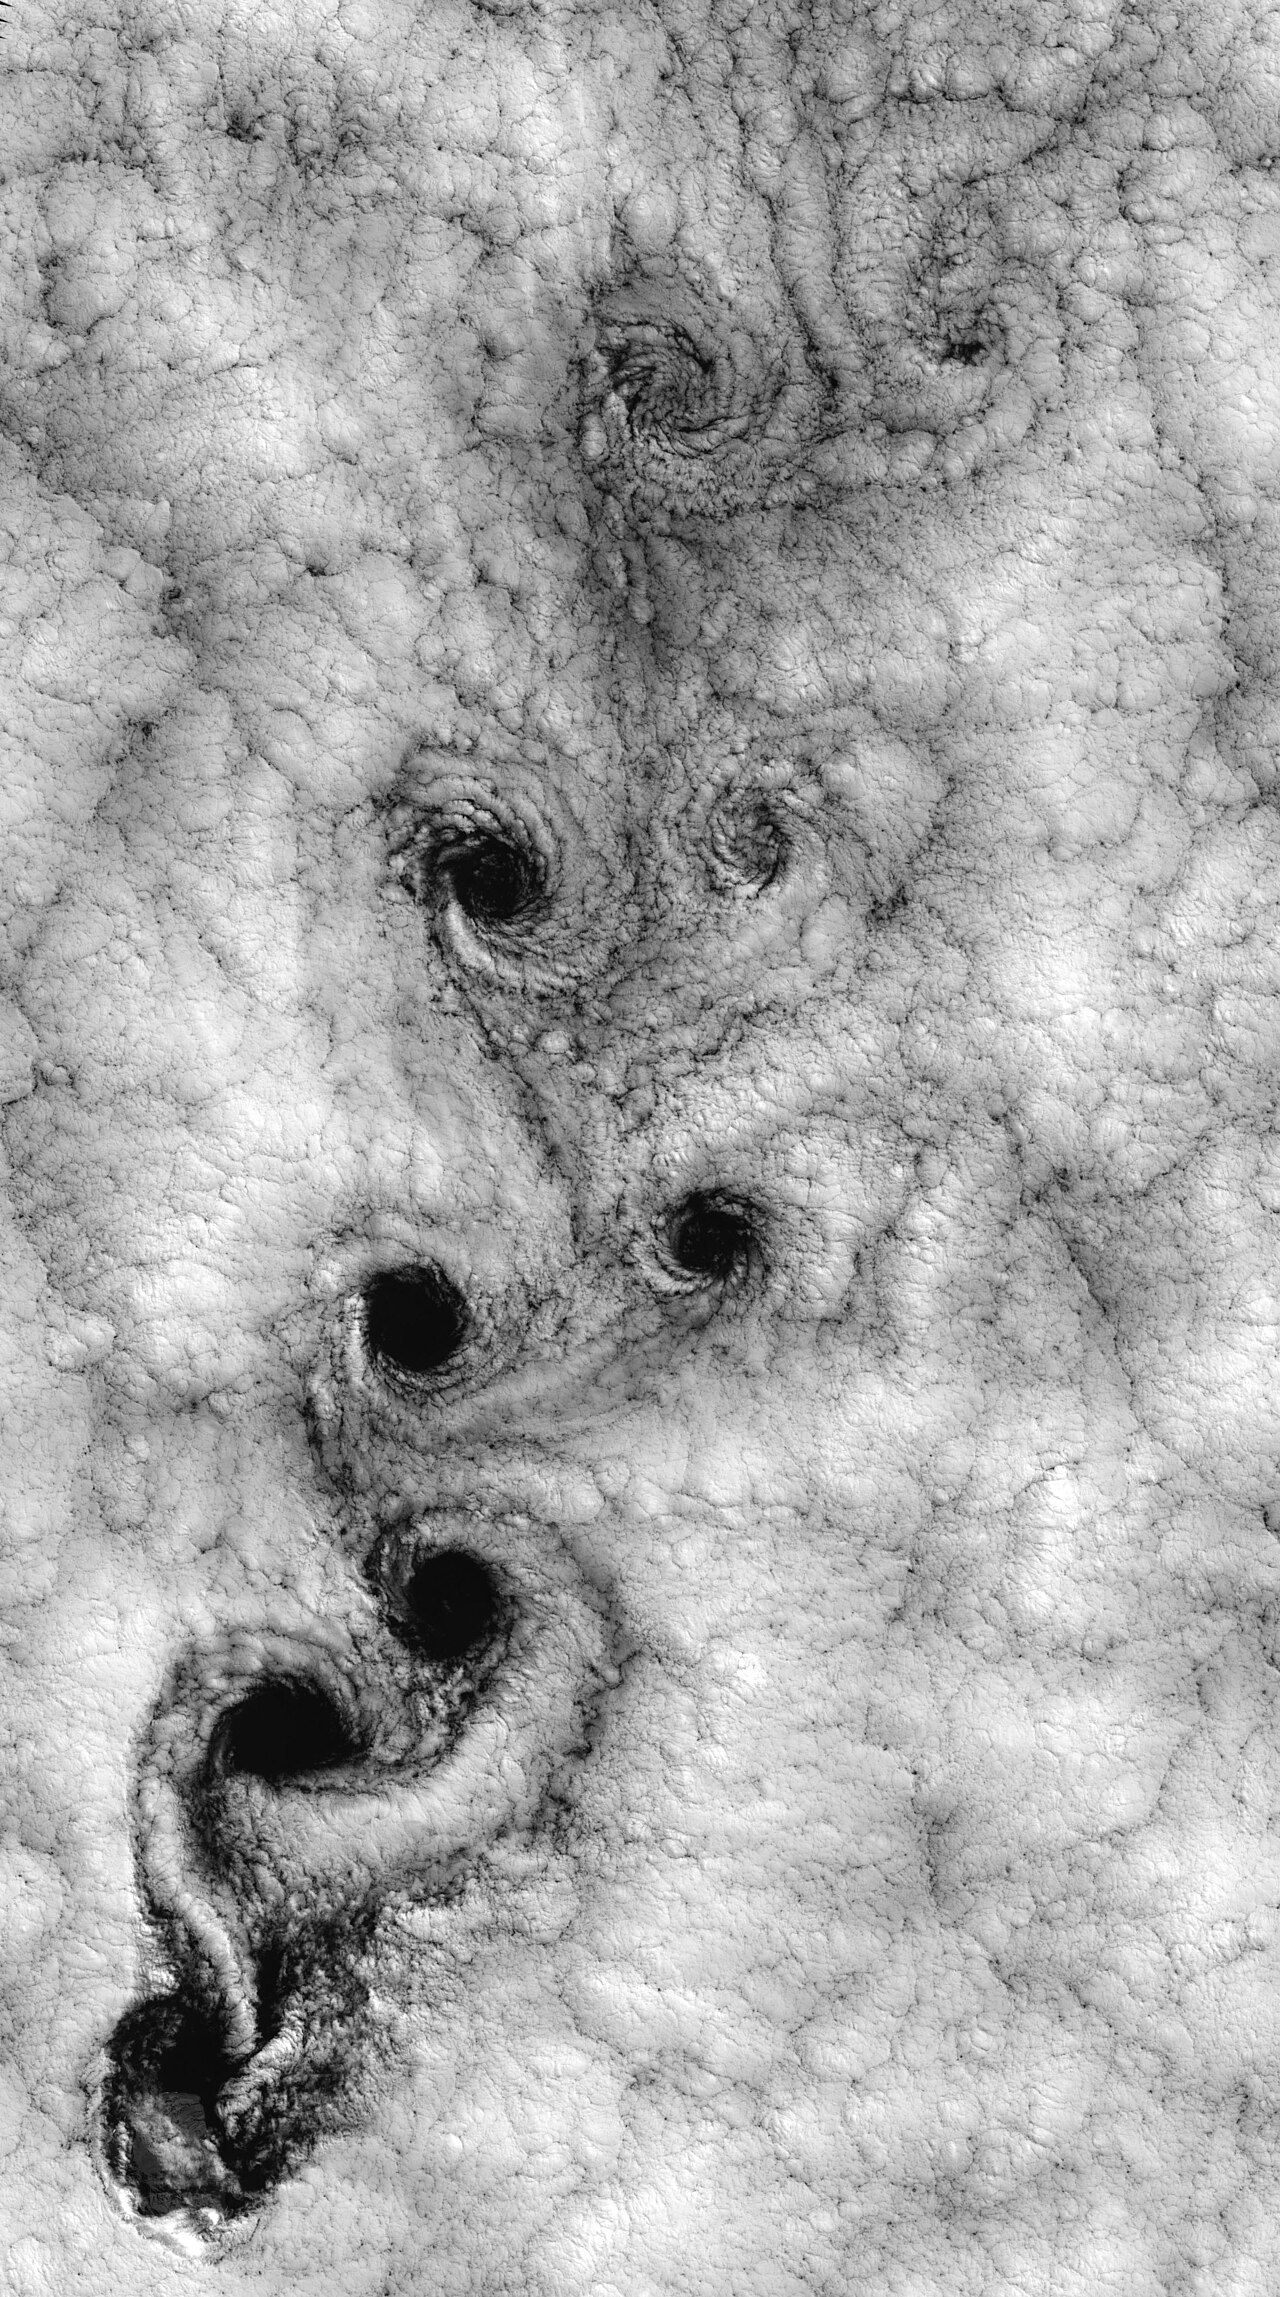
\includegraphics[width=0.34\linewidth]{images/book4/karman-vortex-street.jpg}

{\small Uma rua de vórtices de von Kármán nas nuvens a jusante de uma ilha, vista do espaço: a esteira de um cilindro a um \omterm{def:b2:viscous-flows:reynolds}{número de Reynolds} de algumas centenas, desenhada na escala de uma centena de quilômetros (NASA).}
\end{omfigure}

\section{Problema: Sangue, petróleo e chuva}

\begin{problem}[{Problema de fim de semana --- as mesmas leis viscosas numa artéria,
num oleoduto de mil quilômetros e numa gota que cai}]
\label{pb:b2:viscous-flows:1}

\medskip
\noindent\textbf{Parte I --- O sangue.}
Sangue: $\rho = \qty{1060}{kg/m^3}$, $\eta = \qty{3.5e-3}{Pa.s}$ (tratado como
newtoniano); débito cardíaco $D_V = \qty{5.0}{L/min}$.
\begin{enumerate}
  \item Aorta, raio \qty{1.25}{cm}: celeridade média, \omterm{def:b2:viscous-flows:reynolds}{número de Reynolds}, regime.
  \item Se o escoamento na aorta fosse o de Poiseuille, quais seriam a
        celeridade máxima e a \omterm{def:b2:viscous-flows:viscosity}{tensão de cisalhamento} na parede? (O endotélio
        percebe tensões da ordem de \qty{1}{Pa}.)
  \item Um capilar de raio \qty{4.0}{\micro m} conduz sangue a
        \qty{0.30}{mm/s}: \omterm{def:b2:viscous-flows:reynolds}{número de Reynolds}; queda de pressão ao longo de seu
        comprimento de \qty{1.0}{mm}, em pascals e em milímetros de mercúrio
        (\qty{1}{mmHg} = \qty{133}{Pa}).
  \item Tempo que uma hemácia leva para atravessar o capilar; por que essa é a
        ordem certa para as trocas gasosas?
  \item Arteríolas (raio \qty{10}{\micro m}, comprimento \qty{2.0}{mm}, $10^8$
        em paralelo): resistência do conjunto e queda de pressão
        nele, no débito cardíaco pleno.
  \item A queda total, do lado arterial ao venoso, vale \qty{13}{kPa}: potência
        mecânica entregue pelo ventrículo esquerdo. Compare com um
        corpo de \qty{100}{W}.
  \item Uma estenose reduz em $40\%$ o raio de uma artéria coronária
        num trecho curto: fator pelo qual sua resistência aumenta; por que
        o músculo cardíaco a jusante ainda pode ser irrigado em repouso, mas
        não durante o esforço.
  \item Num esforço intenso o débito cardíaco chega a \qty{25}{L/min}:
        \omterm{def:b2:viscous-flows:reynolds}{número de Reynolds} na aorta, e regime.
  \item O sangue não é newtoniano: sua \omterm{def:b2:viscous-flows:viscosity}{viscosidade} aparente cai a alta
        taxa de cisalhamento e sobe a baixa. Qual dos vasos acima é
        o mais afetado, e em que sentido?
\end{enumerate}

\medskip
\noindent\textbf{Parte II --- O oleoduto.}
Um oleoduto de petróleo bruto: diâmetro $D = \qty{1.2}{m}$, comprimento $L = \qty{1300}{km}$,
vazão $D_V = \qty{3.0}{m^3/s}$; óleo com $\rho = \qty{850}{kg/m^3}$, $\eta =
\qty{2.0e-2}{Pa.s}$ quando mantido aquecido. Atrito turbulento: $\Delta P = \lambda
(L/D)\tfrac12\rho\langle v\rangle^2$, $\lambda = 0.316/\mathrm{Re}^{1/4}$.
\begin{enumerate}[resume]
  \item Celeridade média e \omterm{def:b2:viscous-flows:reynolds}{número de Reynolds}; regime.
  \item Queda de pressão por quilômetro e ao longo de toda a linha.
  \item O tubo suporta \qty{80}{bar}: número mínimo de estações de bombeamento
        ao longo da linha.
  \item Potência total de bombeamento; energia por metro cúbico de óleo entregue,
        comparada com o conteúdo energético do óleo (\qty{36}{GJ/m^3}).
  \item Que queda a lei de Poiseuille preveria? Comente o custo
        da turbulência (e por que aditivos poliméricos que retardam
        a turbulência são injetados em alguns oleodutos).
  \item No inverno o óleo sem aquecimento chegaria a $\eta = \qty{2.0}{Pa.s}$:
        novo \omterm{def:b2:viscous-flows:reynolds}{número de Reynolds} e regime; queda de pressão ao longo da linha
        com a lei apropriada. Conclusão para o projeto (a linha real
        é isolada e o óleo mantido aquecido).
  \item Tempo de trânsito do óleo de uma ponta à outra.
  \item \omterm{def:b2:viscous-flows:viscosity}{Tensão de cisalhamento} na parede no caso quente e turbulento, a partir da
        queda de pressão; \omterm{def:b2:rigid-body-mechanics:contact}{força de atrito} total sobre a parede do tubo.
  \item A mesma vazão num tubo de \qty{1.0}{m}: por que fator muda a
        queda de pressão turbulenta?
  \item Um grão de areia de \qty{0.10}{mm} ($\rho_s = \qty{2650}{kg/m^3}$) é carregado
        pelo óleo quente: celeridade de sedimentação de Stokes, \omterm{def:b2:viscous-flows:reynolds}{número de Reynolds} do
        grão, tempo para decantar a seção do tubo. Compare com as
        flutuações turbulentas de velocidade, alguns por cento de $\langle v
        \rangle$: a areia decanta no oleoduto em operação? E num
        parado?
\end{enumerate}

\medskip
\noindent\textbf{Parte III --- Gotas.}
Ar: $\rho = \qty{1.2}{kg/m^3}$, $\eta = \qty{1.8e-5}{Pa.s}$; água com $\rho_w =
\qty{1000}{kg/m^3}$, $\gamma = \qty{0.072}{N/m}$.
\begin{enumerate}[resume]
  \item Gotícula de nuvem, diâmetro \qty{10}{\micro m}: celeridade terminal de Stokes,
        \omterm{def:b2:viscous-flows:reynolds}{número de Reynolds}, tempo para cair \qty{1}{km}; por que a nuvem permanece.
  \item Garoa, \qty{0.20}{mm}: celeridade de Stokes e \omterm{def:b2:viscous-flows:reynolds}{número de Reynolds}; Stokes
        ainda é confiável?
  \item Gota de chuva, \qty{2.0}{mm}: mostre que Stokes falha e ache a celeridade
        terminal com $C_x = 0.5$. Tempo para cair de \qty{1}{km}.
  \item Numa corrente ascendente de \qty{1}{cm/s}, a gotícula de nuvem sobe ou
        desce? Que corrente ascendente sustentaria a gota de garoa?
  \item \omterm{rem:b2:viscous-flows:capillarity}{Pressão de Laplace} dentro das três gotas; compare com a
        \omterm{thm:b2:euler-bernoulli:bernoulli}{pressão dinâmica} $\tfrac12\rho v_\infty^2$ de cada uma e explique por que
        gotas de chuva grandes se achatam e se rompem acima de cerca de \qty{5}{mm}.
  \item Numa tabela, dê para os oito escoamentos deste problema o
        \omterm{def:b2:viscous-flows:reynolds}{número de Reynolds} e a lei que o governa.
\end{enumerate}
\end{problem}
